%  !TeX  root  =  user_guide.tex

\chapter{Come iniziare}\label{label_getstarted}

% when the revision of a section has been finalized, 
% comment out the following line:
% \updatedisclaimer

Questo capitolo fornisce una veloce panoramica sull'installazione
di \qg, su alcuni dati campione scaricabili dal sito \qg e su come avviare
una prima semplice sessione in cui visualizzare layer raster
e vettoriali.

\section{Installazione}\label{label_installation}
\index{installazione}

L'installazione di \qg è molto semplice. Pacchetti standard per l'installazione
sono disponibili per MS Windows e Mac OS X. Per le distribuzioni GNU/Linux
sono disponibili pacchetti binari (rpm e deb) o archivi software
da aggiungere al gestore di installazione. Informazioni aggiornate
possono essere reperite sul sito web di \qg \url{http://download.qgis.org}.

\minisec{Installazione da codice sorgente}

Se si rende necessario compilare \qg da codice sorgente si può fare riferimento alla guida 
per la compilazione disponibile su \url{http://www.qgis.org/en/documentation/manuals.html}.
Le istruzioni per l'installazione sono anche distribuite con il codice sorgente di \qg.

\minisec{Installazione su supporti esterni}

QGIS permette di specificare un'opzione di percorso (--configpath) che sovrascrive 
il percorso predefinito (es. ~/.qgis in Linux) per le configurazioni utente. 
In tal modo è possibile portare l'installazione di QGIS, comprensiva dei plugin 
e delle impostazioni, su un supporto di memoria esterno (es. penna USB). 

\section{Dati campione}\label{label_sampledata}
\index{data!esempi} 

La guida utente contiene esempi basati sul set di dati campione di
\qg.

\win L'installer per Windows comprende un'opzione per scaricare il
set di dati campione di \qg. Se selezionato, i dati verranno scaricati
nella vostra cartella \filename{Documenti} e posizionati in
una cartella denominata \filename{GIS Database}. Si può usare
Windows Explorer per spostare questa cartella in qualunque altra
posizione. Qualora non fosse stata selezionata l'opzione per installare
il set di dati campione durante l'installazione iniziale di \qg è
possibile: 
\begin{itemize}[label=--]
\item usare dati GIS già posseduti; 
\item scaricare il set di dati dal sito di \qg \url{http://download.qgis.org};
oppure 
\item disinstallare \qg e reinstallarlo selezionando l'opzione per lo scaricamento
dei dati, solo se la soluzione precedente non ha successo. 
\end{itemize}

\nix \osx Per GNU/Linux e Mac OSX non sono ancora disponibili pacchetti
di installazione del set di dati campione in formato rpm, deb or dmg.
Per usare il set di dati campione scaricare il file \filename{qgis\_sample\_data}
come archivio ZIP o TAR da \url{http://download.osgeo.org/qgis/data/}
e decomprimerlo sul vostro sistema. Il dataset Alaska include tutti
i dati GIS usati come esempi e schermate nella guida utente, includendo 
anche un piccolo database GRASS. La proiezione usata per
il set di dati di \qg è Alaska Albers Equal Area con unità in piedi.
Il codice EPSG di questa proiezione è 2964.

\begin{verbatim}
PROJCS["Albers Equal Area",
    GEOGCS["NAD27",
        DATUM["North_American_Datum_1927",
            SPHEROID["Clarke 1866",6378206.4,294.978698213898,
                AUTHORITY["EPSG","7008"]],
            TOWGS84[-3,142,183,0,0,0,0],
            AUTHORITY["EPSG","6267"]],
        PRIMEM["Greenwich",0,
            AUTHORITY["EPSG","8901"]],
        UNIT["degree",0.0174532925199433,
            AUTHORITY["EPSG","9108"]],
        AUTHORITY["EPSG","4267"]],
    PROJECTION["Albers_Conic_Equal_Area"],
    PARAMETER["standard_parallel_1",55],
    PARAMETER["standard_parallel_2",65],
    PARAMETER["latitude_of_center",50],
    PARAMETER["longitude_of_center",-154],
    PARAMETER["false_easting",0],
    PARAMETER["false_northing",0],
    UNIT["us_survey_feet",0.3048006096012192]]
\end{verbatim}

Se s'intende usare \qg come interfaccia per GRASS, sono disponibili delle LOCATION
campione (ad es. Spearfish or South Dakota) sul sito ufficiale
di GRASS GIS  \\
\url{http://grass.osgeo.org/download/data.php}.

\subsection{Sessione di esempio}\label{samplesession}

Ora che si è installato \qg e si ha a disposizione un set di dati
campione, dimostreremo una breve e semplice sessione di \qg. Visualizzeremo
un layer raster ed uno vettoriale. Useremo il layer raster dell'uso
del suolo \filename{qgis\_sample\_data/raster/landcover.img} e
il layer vettoriale dei laghi \filename{qgis\_sample\_data/gml/lakes.gml}.

\minisec{Avvio di \qg}

\begin{itemize}[label=--]
\item \nix {Avviare \qg scrivendo: \usertext{\qg} al prompt dei comandi, oppure 
se si utilizzano pacchetti binari precompilati, utilizzando il menu delle applicazioni.} 
\item \win {Avviare \qg usando il menu Start o l'icona sul desktop, oppure
facendo doppio click su un file di progetto \qg.} 
\item \osx {Doppio click sull'icona nella cartella Applicazioni.}
\end{itemize} 

\begin{figure}[ht]
   \centering 
   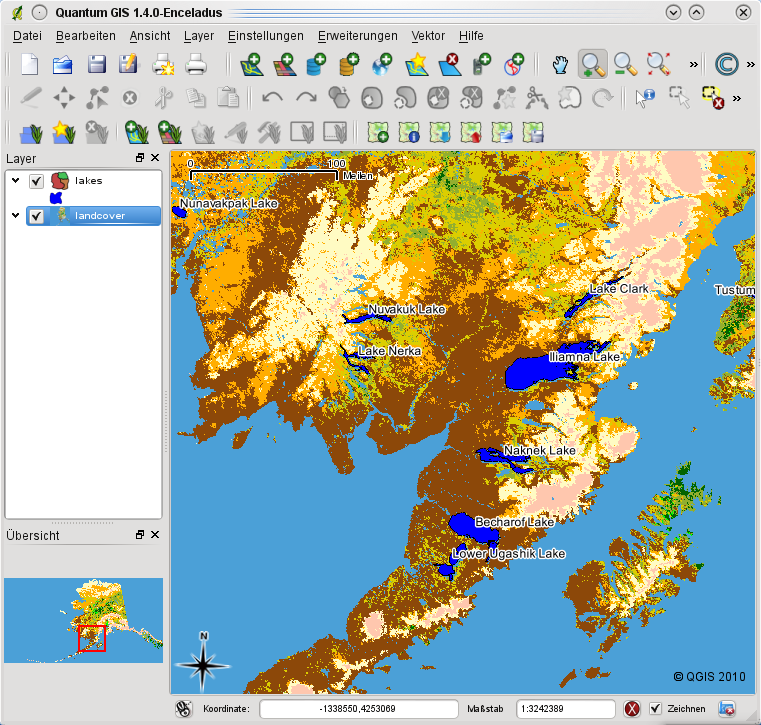
\includegraphics[clip=true, width=12cm]{simple_session}
   \caption{Una sessione di esempio in \qg \nixcaption}\label{fig:simple_session}
\end{figure}

\minisec{Caricare dati raster e vettoriali dal set di dati campione}

{\setlength{\baselineskip}{1.3\baselineskip}
\begin{enumerate}[itemsep=2pt]
\item Cliccare sull'icona \toolbtntwo{mActionAddRasterLayer}{Aggiungi raster}. 
\item Individuare la cartella \filename{qgis\_sample\_data/raster/},
selezionare il file ERDAS Img \filename{landcover.img} e cliccare
\button{Apri}. 
\item Se il file non appare nella lista, controllare se il tipo di file selezionato 
nel menu in basso della finestra di dialogo è corretto, in questo caso "Immagine ERDAS (*.img, *.IMG)"
\item Ora cliccare sull'icona \toolbtntwo{mActionAddOgrLayer}{Aggiungi vettore}. 
\item \radiobuttonon{'File'} deve essere selezionato come tipo di sorgente nella
finestra di dialogo \dialog{Aggiungi vettore}. Ora cliccare \button{Sfoglia} per selezionare il 
layer vettoriale.
\item Individuare la cartella \filename{qgis\_sample\_data/gml/}, selezionare "GML" 
dal menu tipo file, poi selezionare il file GML \filename{lakes.gml} 
e cliccare \button{Apri}, poi nella finestra di dialogo Aggiungi vettore cliccare \button{OK}. 
\item Ingrandire un la vista su un'area a vostra scelta con alcuni laghi. 
\item Fare doppio click sul layer \filename{lakes} nella legenda per
aprire la finestra \dialog{Proprietà layer}. 
\item Cliccare sulla scheda \tab{Stile} e selezionare blu come
colore di riempimento. 
\item Cliccare sulla scheda \tab{Etichette} e spuntare l'opzione \checkbox{Mostra
etichette} per abilitare l'etichettatura. Scegliere il campo NOME come campo per l'etichetta.
\item Per migliorare la leggibilità dell'etichetta, è possibile aggiungere un contorno con sfondo colorato:
spuntare \checkbox{Contorno etichette} e scegliere dimensione e colore del contorno.
\item Cliccare \button{Applica}, controllare se il risultato è buono ed infine 
premete il tasto \button{OK}.
\end{enumerate} 

Visto come è facile visualizzare layer raster e vettoriali in \qg?
Proseguiamo alla sezione seguente per imparare ulteriori funzioni, caratteristiche ed impostazioni.

\FloatBarrier